\documentclass[12pt,letterpaper,noanswers]{exam}
\usepackage[usenames,dvipsnames,svgnames,table]{xcolor}
\usepackage[margin=0.9in]{geometry}
\renewcommand{\familydefault}{\sfdefault}
\usepackage{multicol}
\pagestyle{head}
\header{AM 111 Class 09}{}{Piecewise interpolation, p.\thepage}
\runningheadrule
\headrule
\usepackage{siunitx}
\usepackage{graphicx} % more modern
\usepackage{amsmath} 
\usepackage{amssymb} 
\usepackage{hyperref}
\usepackage{tcolorbox}
\usepackage{enumitem}
\def\mbf{\mathbf}
\newcommand{\vc}[1]{\boldsymbol{#1}}
\def\dsst{\displaystyle}
\DeclareMathOperator*{\argmin}{arg\,min} % thin space, limits underneath in displays


\begin{document}
 \pdfpageheight 11in 
  \pdfpagewidth 8.5in

\noindent 

\section*{Preliminaries}

\begin{itemize}
\itemsep0pt
\item The problem set is due on Friday at 5pm (submit via Gradescope: include pdfs of all code/output on Gradescope.  Upload any source code to Canvas).
\item The problem set includes some ``time permitting'' problems.  If your total time spent on the course outside of class reaches 10 hours in the week then you are encouraged to skip problems.  If you are not in that situation, you are expected to complete the problems.
\item If you need guidance or help on the problem set, post to Ed.
\item There will be a skill check in class during the next class.  The problem info is below.
\item Quiz info is on Canvas.
\end{itemize}



\noindent\textbf{Big picture}

Today: Algorithms for finding a piecewise polynomial that directly passes through data points.

\vspace{0.2cm}
\hrule
\vspace{0.2cm}

\noindent \textbf{Skill check practice}
\begin{questions}
\item 
REDO THE SKILL CHECK WITH A SKILL FROM SAUER \S 3.4...

Use Lagrange interpolation to construct an approximation to $f(x) = \sqrt{x}$ based on the following data points: $(0,0)$,$(4,2)$, $(9,3)$.

Identify the degree of your interpolating polynomial.

\item The skill from the Class 06 handout (Skill Check C07).
\end{questions}


\vspace{0.2cm}
\hrule
\vspace{0.2cm}

\noindent \textbf{Skill check solution}
\begin{questions}
\item First construct the basis functions:

$l_1(x) = \frac{(x-4)(x-9)}{(0-4)(0-9)}$


$l_2(x) = \frac{(x-0)(x-9)}{(4-0)(4-9)}$


$l_3(x) = \frac{(x-0)(x-4)}{(9-0)(9-4)}$

Then construct the polynomial interpolant:
$P(x) = 0l_1(x) + 2l_2(x) + 3l_3(x)$

It turns out that if $y_i = 0$ then there is no need to construct $l_i$.

This polynomial is degree $2$.

\item See the past handout.
\end{questions}
\vspace{0.2cm}
\hrule
\vspace{0.2cm}

\noindent \textbf{Teams}
\begin{multicols}{3}
1. Eletria, Benjamin, Marissa

2. Cameron, Basil, Emma

3. RH, Eric, Esmé

4. Nini, Ray, Dani

5. Jack, Mina, Ivonne

6. Alex, KevinG, Shang

7. Jessica, Johan, Tom

8. Nina, Robert, Padraig

9. KevinC, Alex, Eli

10.  Aidan, Daniyal, Zachary

11. Ghedion, JuliaK, JuliaM

12. Mack, Brian

13. Caitlin, Sophie

\end{multicols}

\section*{Piecewise polynomial interpolation (splines)}

(Koumoutsakos et al lecture 4)

Using a high degree polynomial to interpolate data (as happens in the problems above when $N$ is larger), means the polynomial is likely to be highly oscillatory.  The polynomial may not look like the function being approximated from the sample points.

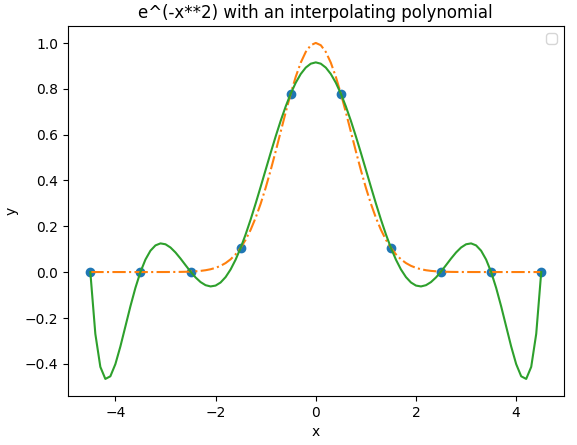
\includegraphics[width=0.5\textwidth]{img/C08gaussinterp.png}

\begin{tcolorbox}
Fit a polynomial to the data piecewise (using just a few data points at a time).

\textbf{Splines} are piecewise polynomials with different parameters in different intervals.
\end{tcolorbox}

% 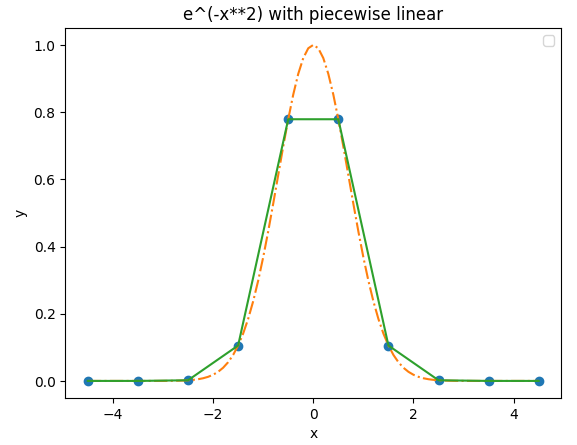
\includegraphics[width=0.5\textwidth]{img/C08linearpiece.png}
% 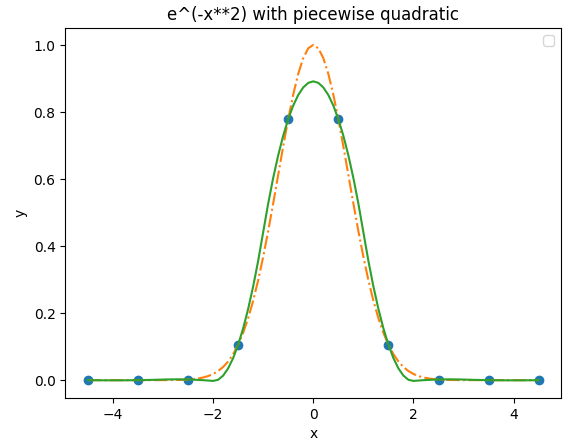
\includegraphics[width=0.5\textwidth]{img/C08picequad.png}

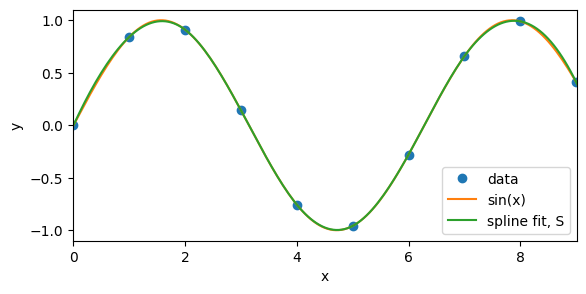
\includegraphics[width=0.5\textwidth]{img/Class09sinspline.png}
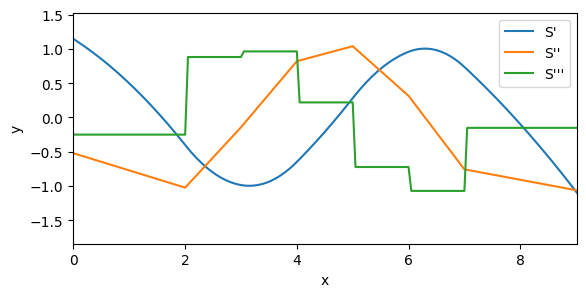
\includegraphics[width=0.5\textwidth]{img/Class09deriv.png}

\begin{enumerate}[resume=classQ]
\item $\sin x$ is shown above with a spline fit, $S$.  On the right are plotted $S', S'',S'''$.  



The spline fit, $S(x) = \left\{\begin{array}{l l} S_1(x) & x_0\leq x < x_1 \\
S_2(x) & x_1\leq x < x_2 \\
\vdots \\
S_k(x) & x_{k-1}\leq x < x_k \\
\end{array}\right.$
\begin{parts}
\item Using the graphs, identify the degree of $S_j(x)$.
\vspace{1cm}

\item Using the graphs, find $k$ (the total number of pieces for the piecewise function).

\vspace{1cm}

\item Is $S$ a continuous function?  Is it differentiable?  How do you know?

\emph{This question is about $S$, and not about its components $S_j$.}
\vspace{1cm}

\end{parts}
\end{enumerate}

\subsection*{Cubic splines}
\begin{tcolorbox}
Start with a dataset $\{(x_i,y_i)\}_{i=0}^N$ with $x_i < x_{i+1}$.  For every interval $[x_{i-1},x_i]$, $i=1,...,N$, define a cubic polynomial \[f_i(x) = \alpha_i x^3 + \beta_i x^2 + \gamma_i x + \delta_i.\]

Let $f(x) = \left\{\begin{array}{l l} f_1(x) & x_0\leq x < x_1 \\
f_2(x) & x_1\leq x < x_2 \\
\vdots \\
f_N(x) & x_{N-1}\leq x < x_N \\
\end{array}\right.$

Find coefficients such that $f$ is a continuous function and $f(x_i) = y_i$.
\end{tcolorbox}
\begin{enumerate}[resume=classQ]
\item 
\begin{parts}
\item How many unknowns are there in the definition of $f(x)$?
\vspace{1cm}

\item How many constraints arise from imposing $f(x_i) = y_i$ and continuity?

\emph{Consider how many equations are needed for each $f_i$ for there to be continuity.}
\vspace{1cm}

\item How many more constraints are needed to uniquely identify the unknowns?
\vspace{1cm}

\end{parts}
\end{enumerate}

\noindent\textbf{More constraints}
\begin{tcolorbox}
Impose continuity on the first and second derivatives: 
\[\begin{array}{l}
f_i'(x_i) = f_{i+1}'(x_i) \\
f_i''(x_i) = f_{i+1}''(x_i)
\end{array}, \quad i = 1,...,N-1\]
\end{tcolorbox}
\begin{enumerate}[resume=classQ]
\item How many additional constraints is this?  How many more are needed?
\vspace{1cm}

\end{enumerate}
\noindent\textbf{Final parameters}
\begin{tcolorbox}
The choice of additional constraints can depend on the problem.  Here are a few options:
\begin{itemize}
\itemsep0pt
    \item natural splines: set $f_1''(x_0) = f_N''(x_N) = 0$
    \item ``not-a-knot'': 1st segments ($f_1$ and $f_2$) and last ($f_{N-1}$ and $f_N$) have the same cubic
    \item parabolic runout: set $f_1''(x_0) = f_1''(x_1)$ and $f_N''(x_N) = f_N''(x_{N-1})$
    \item clamping: set $f_1'(x_0) = f_N'(x_N) = 0$
    \item periodic: set $f_1'(x_0) = f_N'(x_N)$ and $f_1''(x_0) = f_N''(x_N)$
\end{itemize}
\end{tcolorbox}

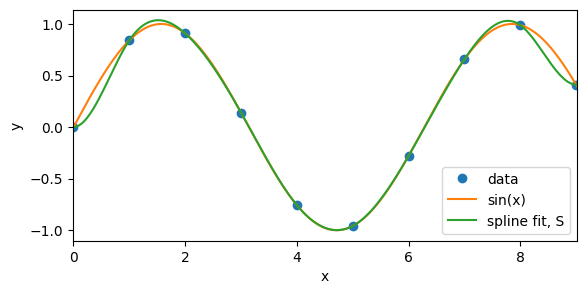
\includegraphics[width=0.5\textwidth]{img/Class09clamp.png}
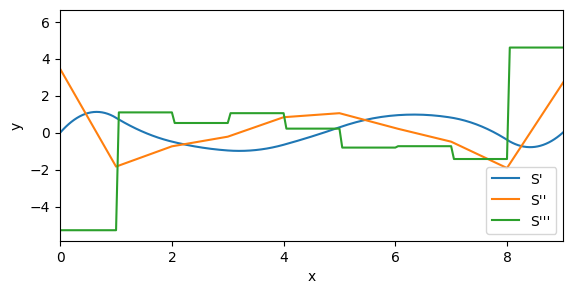
\includegraphics[width=0.5\textwidth]{img/Class09clampderiv.png}

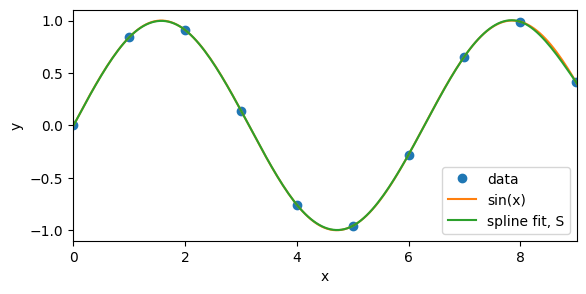
\includegraphics[width=0.5\textwidth]{img/Class09natural.png}
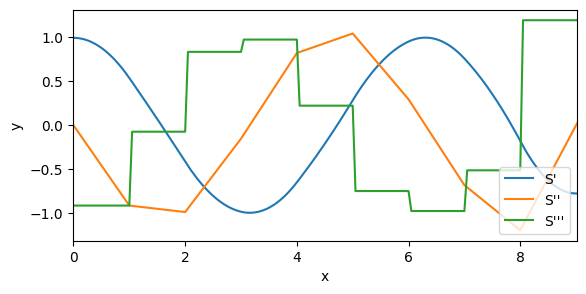
\includegraphics[width=0.5\textwidth]{img/Class09naturalderiv.png}

\begin{enumerate}[resume=classQ]
    \item Three different spline fits to $\sin x$ are given (A: p.2, B: top of this page, C: 2nd on this page)  Match each of them to one of the ways of setting additional constraints.
    
    \emph{How did you make your matches?}
    
    \vspace{1cm}
    
    \item Provide the constraint equations associated with ``not-a-knot''.

    
\end{enumerate}

\subsection*{Finding coefficients}

REDO THIS SECTION TO FOLLOW SAUER \S 3.4...

\begin{tcolorbox}
Instead of using \[f_i(x) = \alpha_i x^3 + \beta_i x^2 + \gamma_i x + \delta_i\]
we'll set up a different form of $f_i$ to find the cubic equations on each segment.  Let \[f_i''(x) = \frac{a_{i-1}}{\Delta x_i}(x_i-x) + \frac{a_i}{\Delta x_i}(x-x_{i-1})\]
with $\Delta x_i = x_i-x_{i-1}$ for $i=1,...,N-1$.
\end{tcolorbox}
\begin{enumerate}[resume=classQ]
\item 
\begin{parts}
\item Evaluate $f_i''(x)$ at $x_i$.
\vspace{1cm}

\item Write down $f_{i+1}''(x)$ and then find $f_{i+1}''(x_i)$.  
\vspace{1cm}

\item Does this construction give continuity of the second derivative?
\vspace{1cm}
\end{parts}
\end{enumerate}
\begin{tcolorbox}
\[f_i'(x) = -\frac{a_{i-1}}{2\Delta x_i}(x_i-x)^2 + \frac{a_i}{2\Delta x_i}(x-x_{i-1})^2+b_i\] is the integral of $f_i''(x)$.

Integrating again generates $f_i(x)$ of the form
\[f_i(x) = \frac{a_{i-1}}{6\Delta x_i}(x_i-x)^3 + \frac{a_i}{6\Delta x_i}(x-x_{i-1})^3+b_i(x-x_{i-1})+ c_i\]

Use $f_{i}(x_{i-1}) = y_{i-1}, f_{i}(x_{i}) = y_{i}$ to find $b_i$ and $c_i$ in terms of the $a_i$.

See Koumoutsakos et al for detailed steps.

This results in $b_i = \frac{\Delta y_i}{\Delta x_i} - \frac{a_i-a_{i-1}}{6}\Delta x_i$ and $c_i = y_{i-1} - \frac{a_{i-1}}{6}\Delta x_i^2$ with $\Delta y_i = y_i - y_{i-1}$.

Using $f_i'(x_i) = f_{i+1}'(x_i)$ leads to a relationship between the $a_i$:
\[a_{i-1}\Delta x_i + a_i (2(\Delta x_i + \Delta x_{i+1}) + a_{i+1} \Delta x_{i+1} = 6\frac{\Delta y_{i+1}}{\Delta x_{i+1}} - 6\frac{\Delta y_i}{\Delta x_i}\] for $i = 1,...,N-1$
\end{tcolorbox}

\begin{enumerate}[resume=classQ]
\item Choose $a_0 = 0, a_N = 0$ as extra constraints and set up a matrix equation $A\vc{a} = \vc{b}$ to represent the system \[a_{i-1}\Delta x_i + a_i (2(\Delta x_i + \Delta x_{i+1}) + a_{i+1} \Delta x_{i+1} = 6\frac{\Delta y_{i+1}}{\Delta x_{i+1}} - 6\frac{\Delta y_i}{\Delta x_i}\] for $i = 1,...,N-1$

Set $\vc{a} = (a_1,a_2,...,a_{N-1})^T$.  Find $A$ and $b$.
\vspace{1.5in}

\end{enumerate}

\begin{tcolorbox}
A matrix of the form \[\left[\begin{array}{ c c c c c c } 
b_1 & c_1 &  &  & & 0 \\
a_2 & b_2 & c_2 &  &  &  \\
 & a_3 & \ddots & \ddots &  &  \\
 &  &\ddots &  &  & \\
  &  & &  &  & c_{N-1}\\
0 & & & & a_N & b_N
\end{array}\right]\]

is called \textbf{tridiagonal}
\end{tcolorbox}

\begin{enumerate}[resume=classQ]
\item Consider the system \[\left[\begin{array}{c c c c}
1 & 2 & 0 & 0 \\
2 & 3 & 4 & 0 \\
0 & 1 & 7 & 3\\
0 & 0 & 4 & 2
\end{array}\right]\vc{x} = \left[\begin{array}{c} 
1 \\ 6 \\ 7 \\ 2
\end{array}\right]\]

\begin{parts}
\item Eliminate the $a_i$ elements.  Divide the first row by $b_1$, multiply by $a_2$, and subtract if from the second row.  Continue with this procedure to create an upper triangular matrix.
\vfill

\item How many addition, subtraction, multiplication, division operations did this require?  These are basic floating point operations, FLOPs.
\vspace{1cm}

\item Use back substitution to solve your resulting matrix.
\vfill

\item Again count the FLOPs.

\end{parts}

This algorithm for solving a tridiagonal system is $\mathcal{O}(N)$.
\end{enumerate}


\href{https://edsonmarine.com/set-of-six-bronze-spline-weights/}{Splines for sale}
\end{document}